\documentclass[USenglish]{article}

\usepackage[utf8]{inputenc}%(only for the pdftex engine)
%\RequirePackage[no-math]{fontspec}%(only for the luatex or the xetex engine)
\usepackage[small]{dgruyter}
\usepackage{microtype}
\usepackage{graphicx}
\usepackage[style=oscola]{biblatex}
\usepackage{csquotes}
\usepackage{caption}
\usepackage{subcaption}

\bibliography{references.bib}

\begin{document}

  \articletype{Research Article}

  \author*[1]{Johan Pouwelse}
  \author[2]{Martijn de Vos}
  \runningauthor{...}
  \affil[1]{Department of Software Technology, Delft University of Technology}
  \affil[2]{Department of Software Technology, Delft University of Technology}
  \title{Laws for Creating Trust in the Blockchain Age}
  \abstract{...}
  \keywords{Blockchain, Trust, Programmable Economy, Transactions}

\maketitle

\section{Introduction}
Humanity has a disposition to trust, meaning the tendency of individuals to be willing to depend on others.
Technology is altering our notion of trust.
New technology platforms such as Uber and Airbnb disrupt how taxi services are provided and the way in which apartments are rented out.

For these platforms, trust is an essential element: people step into the car of a person they never met before or let strangers sleep in their spare room without worries.
Trust is addressed by rating systems, the foundation for their quality and safety measures.
For instance, pre-testing for potentially dangerous drivers and pre-screening is reduced and replaced with a continuous quality monitoring system\footcite{uberfivestar}.
The Uber mobile application asks both drivers and passengers to provide feedback on their experience.
The software averages the one to five-star ratings of the most recent 500 trips\footcite{uberratinghelp}.
If this average long-term quality rating of a driver drops below a certain level, it automatically triggers contract termination\footcite{forbesuserfiring}. 
The traditional dynamics of trust are altered on such platforms.
Employment regulations are under pressure: some courts found that Uber violated local taxi regulations\footcite{ftuberregulation}\footcite{reutersuberdanish}\footcite{reutersubersouthkorea}.
For the United Kingdom these platforms are responsible for lowering unemployment levels, reducing fixed employment contracts by a few percent, enforce the trend towards zero-hour contracts and self-employment.
A 2017 United Kingdom government report states that currently 1.1 million people work within this gig economy\footcite{goodgigs}.
The laws which govern trust, employment terminations, and access to marketplaces are no longer the exclusive domain of national law.
Laws of trust are now partly inside commercial software.

This work aims to help transform the gig economy.
We aim to institutionalize the empowerment of workers and small businesses with our software, rules and architectural principles.

First, we designed and created an operational open source prototype of the core Uber functionality, matching drivers and passengers on a two-sided market.
Our non-profit alternative aims to be more transparent, fair, and open.
Second, we devised an alternative set of rules and principles for the emergence of trust, using only repeated interactions between strangers.
Third, we present a blueprint for a public infrastructure and prototypes for each part of this blueprint for the gig economy.
Our proposed public infrastructure in principle should be able to offer non-profit alternative to current matchmaking platforms (e.g. Uber, TaskRabbit, Amazon, Expedia, Booking, etc.).
Finally, we hint at how such an infrastructure might be used to realise what has become known as the \emph{programmable economy}.

Blockchain technology is at the core of our proposed Uber alternative and blueprint for a public gig economy.
However, Bitcoin and Ethereum are in our opinion unsuitable for this task or other legal processes such as land registration.
We do not consider cybercurrency research in the remainder of this work.
Our reason is that all current work based on coin creation, blockchain consensus like proof-of-work or variants thereof lack robust and effective ties to any legal system, or even the real world in general.
The current generation of cybercurrency-based blockchain technology lacks a durable governance structure.
Severe disagreements exists within these communities, as various factions battle for control of ecosystems worth billions.
The cybercurrency ecosystem is unsuitable for land registration as it occasionally has periods dubbed civil war by the media\footcite{bloombergbitcoinsplinter}.
We also do not consider private or consortium blockchains, as they do not offer any significant advantage over classical distributed databases.
We focus on the tamper-proof leaderless database type of solutions.
The statements and opinions in this paper are based on our decade-long experience of deploying and gradually improving our own ledger, installed by 1.8 million users.
We deployed a very primitive fully distributed ledger in August 2007, pre-dating the launch of Bitcoin\footcite{bbcnewstribler}.
In 2017 we have mathematically proven that our blockchain technology, TrustChain, scales linear and surpasses a transaction throughput of 10.000 transactions per second\footcite{githubissueconsensus}.

\section{Problem Description}

Contracts, transactions, and the records of them are among the defining structures in our economic, legal, and political systems\footcite{harvardbusinessblockchain}.
They protect assets and set organizational boundaries.
These authentic records create ownership, determine citizenship, and define partnerships between entities.
It establishes a governance layer in which states, economic actors, and citizens interact, effectively creating trust.

For thousands of years trusted guardians kept authentic ownership records of land and assets in general.
These centralized bureaucracies which govern these records have not changed much, while the world is slowly being filled with autonomous cars, trucks, drones, and barges. 
This difference in innovation speed is creating increasing levels of friction around data governance. 
The legal world might be at the beginning of a transition towards full digitization, additional standardization, and further automation. 
Already 22 years ago the book "Law in a Digital World" was published, however deeds of land transfer are rarely pure in digital form\footcite{katsh1995law}.

Blockchain enthusiasts claim this technology offers an alternative to any trusted guardian and central bank.
It offers us another way to organise society, with a high degree of decentralization.
The resilience of Bitcoin together with the rising gig economy endorses this claim.
The breakthrough that made the gig economy possible was the use of reputation systems to build trust between strangers.
Reputation systems collect and process information about past interactions, to help people evaluate the trustworthiness of others\footcite{resnick2002trust}.
However, an individual’s reputation on a platform such as eBay is owned by a profit-driven entity.
This leads to the following problems for the social good:
\begin{itemize}
	\item Lock-in: a solid reputation on one platform is locked into that platform: you cannot move your reputation. Like other forms of lock-in, this inhibits competition and encourages monopoly behaviour. Ironically, companies in the \enquote{sharing economy} do not share reputations. Users are increasingly being protected by European Union law from such data silos. The newly defined right to data portability allows individuals to obtain and reuse their personal data for their own purposes across different services\footcite{dataportabilityeu}.
	\item Fragmentation: each company operates its own closed market, only accessible through their (mobile) application. This leads to lower overall efficiency, compared to a single open market. For example, the ride-hailing market is fragmented into numerous closed markets operated by companies such as Uber, Lyft, BlaBla Car, Didi Kuaidi, GrabTaxi and Karhoo. Each isolated marketplace tries to match drivers and customers in real-time and have to overcome similar challenges.
\end{itemize}
Centralized approaches are ultimately always influenced by the goals and the reliability of the central entity or authority that controls them. 
One economic model even predicts the rise of predatory, monopolistic platforms within two-sided markets\footcite{loertscher2016predatory}.
For this reason, central platforms can never be truly generic and universal. 
With a decentralized approach, multiple independent individuals cooperate in some manner to build a single ecosystem and no one entity has control over the entire environment.
This is the model we envision for the future programmable economy: trust relations are not locked to a single profit-driven entity.

The cardinal problem is: \emph{who owns trust}?
Creating and maintaining trust within a public, shared infrastructure has proven to be a hard problem.
While there is much conducted research on this specific topic, a reliable, secure and real-world deployed trust mechanism stays out.

In May 1962 the vision of a time-sharing computer system with many remote stations was presented, known as the Internet today\footcite{licklider1962line}.
Nobody owns the Internet.
This has been a critical factor for its decades long success story.
The Internet consists of numerous Autonomous Systems which are loosely coupled and have a common numbering mechanism.
On top of this global communication infrastructure we built email, video conferencing, entertainment platforms, search engines, marketplaces, countless cloud services, and essentially a digital economy.
However, these examples often contain a single central point of control and authority.
It has proven to be hard to create a decentralized governance layer for such vital public infrastructure.

Joseph Stiglitz co-authored the "Architecture of Economic Systems" in 1985, describing how decision making units can be organized together within a system\footcite{sah1985architecture}.
It presents a basic framework to compare the performance of decentralized and centralized economic systems.
Centralized economic systems have given way to decentralized forms.
The current challenge is to further refine the decentralized form: storage and governance of authoritative answers to ownership questions using a public and transparent infrastructure.

Trust, accountability, and reputation mechanisms are closely tied.
Transparency can be used to make an authority accountable in order to establish trust. 
It promotes integrity of operations by monitoring the correct behaviour of economic actors\footcite{troncoso2017systematizing}.

Creating trustworthy, public, transparent, and decentralized infrastructures is non-trivial.
We lack a decentral solution for essential economic primitives such as digital identities, money, trust, and marketplaces. 

\section{Architecture for Creating Trust}

We propose an architecture to create a trustworthy decentralized infrastructure for four economic primitives.
The novelty of our work is the application of the Internet architecture throughout our architecture, owned by both everybody and nobody
Our work is academically pure: it relies on self-governance, and weak coupling between autonomous entities. 
Each of the four economic primitives are meticulously designed without relying on any middleman, they are void of any central authority, make traditional intermediaries optional, do not require any central server, remove the need for central databases, and even do not depend on Internet connectivity.

Our blueprint builds heavily on the concepts proven within the gig economy and combines it with blockchain technology.
It contains four layers: strong digital identities, sub-second programmable money transfers, digital trust, and blockchain-regulated marketplaces.
We believe our proposal is the first proposal with real-world viability, as it is the only detailed proposal based on rigorous experimental science: running code.
This work is based on a decade of experimentation: for each component within our architecture we crafted various generations of operational prototypes and conducted Internet-deployment tests.
Each of the four layers in our proposed economic architectural blueprint is designed to reinforce the strength, usability and efficiency of the other layers. 
Upcoming sections present how we applied and validated our architecture by creating a decentralized alternative for Uber and an open, shared market for mortgage financing.

We believe that blockchain technology enables decentralized economies of higher efficiency and stability then currently known. 
This work broadens the applications of the organisational principle behind the Internet, offering full sovereignty to all decision making entities, full transparency on their past performance, and openness in general.
We are applying ideas fundamentally concerned with freedom of individuals, embedding humanities natural disposition to trust, and combining it with a very unforgiving blockchain-based mechanism for rule-breaking economic actors: digital ostracism\footcite{bicchieri2004trust}. 
The threat of being banned forever from an ecosystem may seem to lack compassion and decency, but boosts trust. 
Game theory shows that the "shadow of the future" removes cheating incentives\footcite{friedman1971non}.
Note that fraud differs from blunders by economic actors, which merely impact their reputation (e.g. star rating).
In our architecture we apply the grim trigger defined in 1971 to punish dishonesty, lying, cheating, and fraud.
In other words, mistakes can be forgiven, but intentional digital manipulations are not.

Our work establishes a blueprint for creating a trustworthy, programmable economy.
The term programmable economy was introduced by consultancy firm Gartner Inc. in 2015. 
We expand upon their ideas with various architectural details, propose feasible rules, show operational prototypes, and in general mature this concept.
They describe it as ``the programmable economy, enabled by metacoin platforms and smart technologies, will support new forms of value exchange, new kinds of markets (including dynamically defined on-demand markets), and new kinds of economies such as the attention economy, the reputation economy, the on-demand economy and the resource optimization economy.''\footcite{gartnerprogrammableeconomy}

\begin{figure}[t]
	\centering
	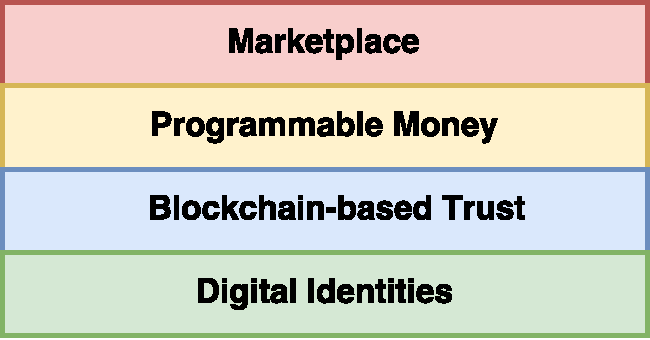
\includegraphics[width=1\columnwidth]{assets/tech_stack_simple}
	\caption{Our four-layered architecture for creating trust.}
	\label{fig:tech_stack_simple}
\end{figure}

Figure \ref{fig:tech_stack_simple} shows the four layers which define our architecture.
First we need to address the digital identity problem, shown as the bottom layer.
A wealth of applications require strong authentication and long-lived secure identities.
The Internet requires a common continuously evolving strong identity layer.
This would make the Internet safer, better and more efficient.
A single common identity layer also needs full decentralization and self-governance.
This blocks progress, for instance, a single standard for globally legally valid electronic signatures which does not yet exist.
This work is motivated by the lack of control over our identity, as formulated within the proposed WebDHT documentation\footcite{webdhtproposal}: 

\blockquote{\enquote{The Web currently does not have a mechanism where people and organizations can claim identifiers that they have sole ownership over. Identifiers, such as those rooted in domain names like emails addresses and website addresses, are effectively rented by people and organizations rather than owned. Therefore, their use as long-term identifiers is dependent upon parameters outside of their control. One danger is that if the rent is not paid, all data associated with the identifier can be made temporarily or permanently inaccessible. This document specifies a mechanism where people and organizations can cryptographically claim ownership over identifiers such that they control them and the documents that they refer to.}}

Self-sovereign identities require that users are the rulers of their own identity.
This idea was presented in 2012 by Moxie Marlinspike\footcite{sovereignsource}.
With this concept people and businesses can store their own identity data on their own devices, and present it efficiently to anyone who wants to validate it.
The decentralized storage within the concept removes the need for any central database of identity data.
This might be increasingly important with the European Union General Data Protection Regulation\footcite{dataportabilityeu}.

This approach to identity is a complete overhaul to the approach used today by governments using central controlled identity administration frameworks.
Users become autonomous by using self-sovereign identities and are free to store their digital passport inside their own smartphone device.
Instead of your government assigning you citizen number "0013" or your telecommunication provider renting you cell phone number "0-013" you can claim ownership of cryptographic key "8A4D48B" as you worldwide identity.
Together with cryptographic techniques it becomes possible to identify and authenticate people, members of organisations and objects without even requiring Internet access.
A large list of worldwide claimed identities by citizens could replace all central identity administration frameworks, increasing efficiency and data portability.

Being the ruler of your own identity is closely related to the core concept of Bitcoin.
Bitcoin creates money without banks, but also provides users with an exceptional level of control.
The novelty of Bitcoin is that is provides a system where nobody can stop a specific entity from spending their money\footcite{r3corda}.
Identity autonomy provides a new level of citizen empowerment and enables financial sovereignty\footcite{matouk2009financial}.

The second layer is our TrustChain fabric, a blockchain design with loose coupling and linear scalability of transaction throughput. 
Our work differs radically from the current generation of cybercurrency, which does not scale beyond several transactions per second. 
We specifically avoid the concept of coins.
TrustChain exclusively focusses on the emergence of trust through repeated interactions.
Instead of using complex mathematical puzzles, our basic building blocks are the interactions between untrusted entities, an idea that naturally extends to the real world.
Each actor within our ecosystem operates their own unique database which contains measures against tampering and makes prior agreed transactions irrefutable.
Within TrustChain each actor is completely autonomous, owns their own chain, and publishes new electronic business transactions in a tamper-proof append-only manner.

TrustChain and all other layers in our architecture utilise a new model of governance that we call self-governance.
It is an ecosystem where ordinary users self-organise into a large-scale Internet-based collective which can be freely joined by anyone, with the special strong property that all authority is temporary.
We define a self-governance system as a distributed system in which autonomous individuals can collectively exercise all of the necessary functions of power without intervention from any authority which they cannot themselves alter.
Self-governance implies a mechanism for peaceful transfer of power. 
Users may directly vote on new laws, changes to rules, routine maintenance updates, and key changes in principles. 
This approach has proven to be usable, but occasionally leads to fascinating outcomes.
On 20 July 2016 the Ethereum community split apart because a majority voted to revert a completely valid transaction, created by faulty user software (known as the DAO hack)\footcite{cryptocomparedao}.
Another option is to use representatives and appoint professionals responsible for the daily administration of the community through some voting process.
However, this goes against the prevailing anti-authority culture within operational blockchain ecosystems.
Distributed systems with self-governance have no external overseers and no central controlling servers.

The third layer in Figure \ref{fig:tech_stack_simple} transforms our usage of money.
Our proposed approach there is again the opposite of the cybercurrency community.
We believe building a trustworthy and reliable financial infrastructure from scratch is unwise.
By re-engineering and building upon existing bank-based payment systems we provide a realistic, legally compliant, and efficient overlay.
We re-use the existing infrastructure and transform it into loosely coupled autonomous entities.
We provide a proof-of-principle prototype for making international money transfers with sub-second speed, near-zero commissions, instant clearance, and real-time settlement. 
Steps towards a programmable economy necessitate a transformation of the expensive transaction network build in 1970s (SWIFT) using a programming language from the 1950s (COBOL)\footcite{scott2017society}.

Our fourth layer consists of a generic value exchange marketplace and coordination mechanism.
This enables efficient, fast, and secure usage of blockchain technology to enable trade at a large scale and coordinate existing businesses.
We provide an open alternative for Uber and evaluate the efficiency of our approach using a real-world dataset.
This layer is focussed on the open market showcased by the gig economy, but also offers the more traditional alternatives like currency exchange.

In a recent economics publication it is stated that with blockchains, marketplaces can be bootstrapped without the need of traditional trusted intermediaries, lowering the cost of networking\footcite{catalini2016some}.
Furthermore they challenge existing revenue models and incumbents's market power, and opens opportunities for novel approaches to regulation, auctions and the provision of public goods, software, identity and reputation systems.
Little experience, evidence, and knowledge exists for devising this fourth layer.
We are currently conducting trials with various businesses to expand our understanding.
This is a new, developing area of research, however, we believe too few research teams have the resources for the learn-by-doing methodology required to make serious scientific progress.
Building open infrastructures with self-governance is costly (our key funding was the EU FP7 project P2P-Next of 19.500.000 Euro\footcite{p2pnextfunding} and QLectives of 6.900.000 Euro\footcite{qlectivefunding}).

\section{Land Registration Application}

Recently the World Bank indicated that 70\% of the world’s population still lacks access to proper land titling or demarcation services\footcite{ieglandadministration}.
A digital land registration system using blockchain technology requires a re-design of existing procedures for submission and verification of records and claims.
It is most likely to demand changes to legal frameworks.

Obtaining agreement from numerous parties during several of the stages of a property transactions, detecting errors, and to preserve tamper-proof logging is a significant challenge.
Central keepers of records are often entrusted with this critical coordination task.
Blockchains clearly have potential here, offering transparency, reducing overhead, and especially providing a single-source-of-truth.
Various reports support this opinion\footcite{deloitteblockchain}.

Our presented architecture for the programmable economy is designed to greatly simplify critical public infrastructure such as land ownership.
As technology experts we are unable to judge if laws of various countries are ready to transition to a world where analog printouts hold less authority and the digital world is the authoritative source of truth.
To date it seems no country recognizes the electronic signatures created using self-sovereign identity systems.

The blockchain technology of today is sufficiently mature to start prototyping and understanding the (possible) advantages for land registration. 
This technology is not yet sufficiently understood to underpin such an essential public service, but it will be soon.
Similar to self-driving cars, it is likely that legal issues will decelerate technological progress.

\section{Open Market for Mortgage Finance}

\begin{figure}[t]
	\centering
	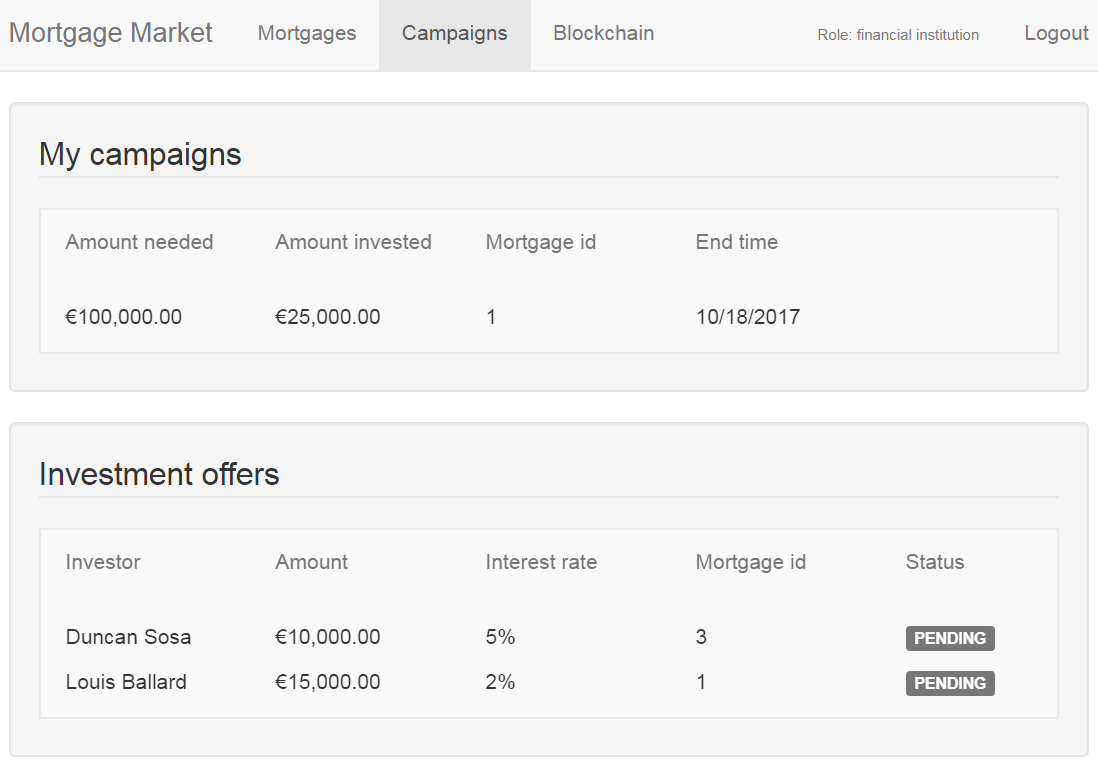
\includegraphics[width=1\columnwidth]{assets/mortgagemarket}
	\caption{The user interface of our mortgage market prototype, from the perspective of an investor.}
	\label{fig:mortgage_market_interface}
\end{figure}

We created a minimal prototype to offer mortgage financing on an open, decentralized and blockchain-regulated market.
Our application enables financial service providers like banks to offer consumers mortgage products and obtain the required capital investments from the global market.
This enables external investors like foreign pension funds to invest in real-estate of financially solid countries with predictable return-on-investment and lower risk.
Traditionally, the mortgage market is inaccessible for the public and nontransparent.
This prototype aims to explore a viable and open alternative to decrease overhead of mortgage processes and offers a real-estate aftermarket where investors can negotiate agreements and trade.
A screenshot of the developed application is presented in Figure \ref{fig:mortgage_market_interface}, showing the user interface from the perspective of a financial institution.

Each agreement reached between individuals in the market are stored as a double-signed contract on a public blockchain.
The mortgage financing platform distinguishes between three different types of contracts:
\begin{itemize}
	\item Mortgage contract: this contract represent the initial mortgage agreement between a user and a mortgage provider, containing all relevant information about the agreed mortgage (i.e. the house address, mortgage rate and redemption agreements).
	\item Investment contract: this type of contract is created when (a part of) a mortgage is sold to an investor. It holds properties of the resold mortgage.
	\item Transaction contracts: when a mortgage is transferred from one investor to another, a transaction contract is created.
\end{itemize}
Investment and transaction contracts are expected to depend on another contract.
For investment contracts, this should be a mortgage contract whereas transaction contracts should have a investment contract as dependency.
Contract dependencies, originating from a single mortgage contract, provide a public overview of all mortgage ownership transferrals since the existence of the mortgage contract.

To store contractual agreements, a blockchain specifically suitable for transactions that transfer ownership of assets between entities, in this scenario, mortgages, has been designed and implemented.
After a contract has been digitally signed by both involved parties, both transaction participants send the contract to all banks (we assume that financial institutions are always available and connected on our platform).
Periodically, banks will try to add a new block, containing one or more received contracts, to the blockchain.
Contracts can only be appended to a transaction block if all of the contract's dependencies are already available on the blockchain.
The adopted consensus mechanism here is proof-of-work: while the scalability of this mechanism is limited, it is viable for our prototype since mortgages won't be created and traded at a high rate.
A dynamic difficulty target mechanism assures that on average, one new block is added to the chain every three minutes.

\section{Technology Portfolio for Trust Creation}

\begin{figure}[t]
	\centering
	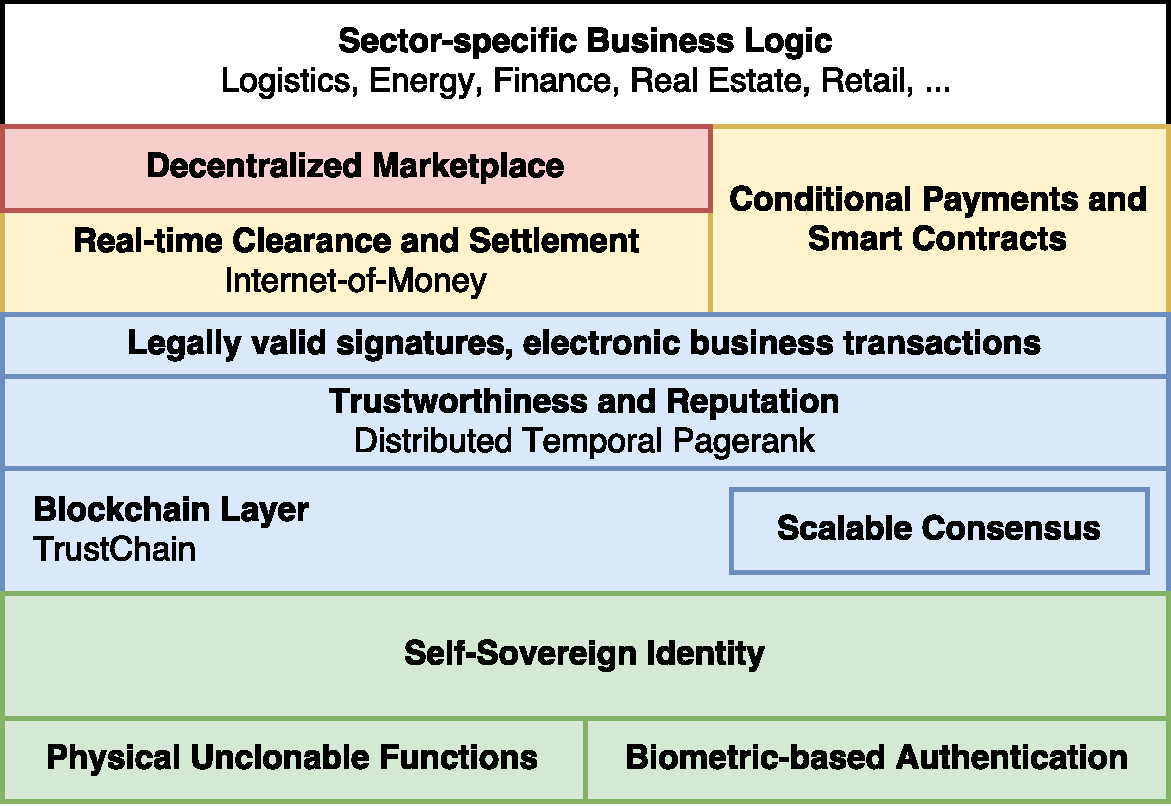
\includegraphics[width=1\columnwidth]{assets/tech_stack}
	\caption{Our detailed technology portfolio for trust creation.}
	\label{fig:tech_stack}
\end{figure}

We now expand on each of the four layers of our envisioned architecture, introduced in Figure \ref{fig:tech_stack_simple}, for a programmable economy.
The detailed architecture of the economic primitives digital identity, trust, programmable money, and marketplaces will be elaborated and is presented in Figure \ref{fig:tech_stack}.

\subsection{Physical Unclonable Functions}
\label{sec:pufs}
Some foundations of security are based on the laws of physics.
For numerous years scientists have searched for a secure basis for critical infrastructure and we believe physical devices provide the desired basis.
We specifically avoid using software and the risk of implementation bugs or weaknesses.
Physical devices for security purposes are already widely used in the cooperate world, mainly as mean to implement a two-factor authentication system.

A Physical Unclonable Function (PUF) is a device that is easy and cheap to produce but practically infeasible to duplicate, due to minor variations in the manufacturing process of the hardware\footcite{cortez2012modeling}.
Their typical usage can be found in applications that require a high level of security, for instance, self-sovereign identity solutions.
The device offers tamper-proof and safe storage of cryptographic keys, representing ones identity.
Each PUF device contains an unique fingerprint, determined by randomness of embedded components.
A PUF responds to challenges and leads to unique but unpredictable responses, together forming a challenge-response pair.
These challenges are often triggered by pushing a physical button attached to the device.

\begin{figure}
	\centering
	\begin{subfigure}{.5\textwidth}
		\centering
		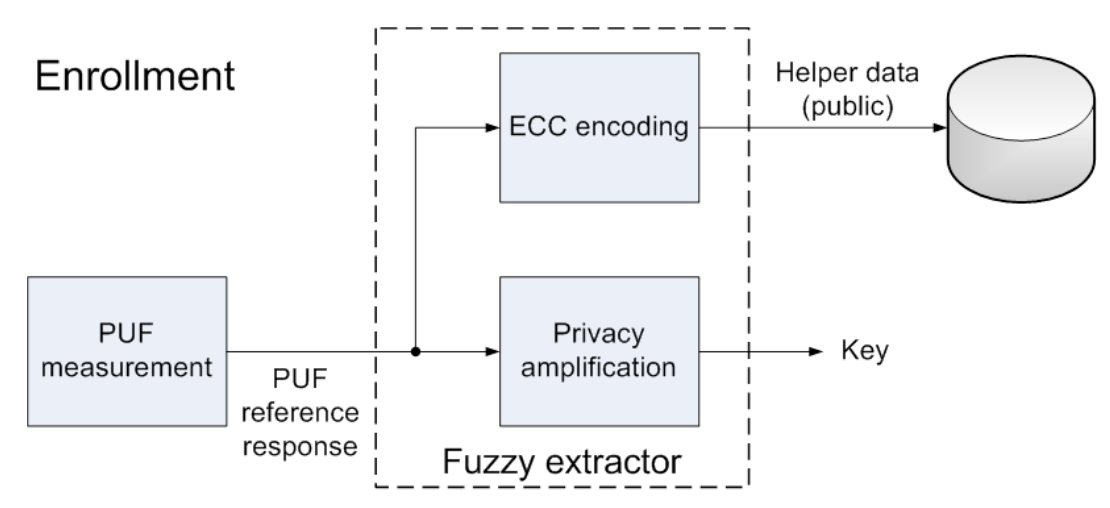
\includegraphics[width=.9\linewidth]{assets/puf_enrollment}
		\caption{Enrollment phase}
		\label{fig:puf_enrollment}
	\end{subfigure}%
	\begin{subfigure}{.5\textwidth}
		\centering
		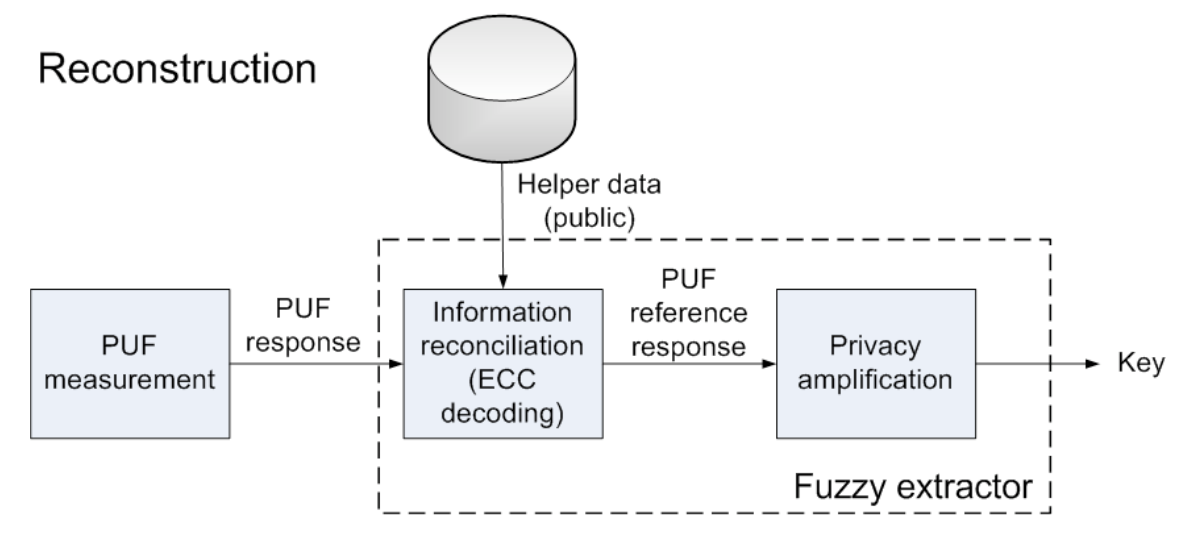
\includegraphics[width=.9\linewidth]{assets/puf_reconstruction}
		\caption{Reconstruction phase}
		\label{fig:puf_reconstruction}
	\end{subfigure}
	\caption{Procedure to store and restore a cryptographic key with a PUF device.}
	\label{fig:puf_key_storage}
\end{figure}

A secure process for identity storage based on a PUF device proceeds in two phases: the enrollment phase (Figure \ref{fig:puf_enrollment}), where a cryptographic key, based on a PUF fingerprint is generated and the reconstruction phase (Figure \ref{fig:puf_reconstruction}), which restores the secret cryptographic key that was generated during the enrollment phase.
Each phase will now be explained according to the Figure \ref{fig:puf_key_storage}.
\begin{itemize}
	\item Enrollment phase: first, a so-called reference response of the targeted PUF is measured after initiating a challenge of the device. This reference response is used as input for the Fuzzy Extractor, which consists of a privacy amplification module and Error-Correcting Code (ECC) encoding. The privacy amplification module converts the PUF reference response to a usable cryptographic key. Additionally, some helper data is computed and saved in storage attached to the device. This helper data itself is not sufficient to restore the secret key and is used during the reconstruction phase.
	\item Reconstruction phase: reconstruction of a stored key starts by measuring the PUF response, which is used as input for the Fuzzy Extractor. The helper data, generated during enrollment, is used to perform information reconciliation and generates the PUF reference response. After privacy amplification, the programmed cryptographic key is restored and ready for usage.
\end{itemize}

PUF devices can also be utilized for identification purposes.
An authentication mechanism based on PUFs works as follows: imagine a bank that needs to identity customers.
For each customer, the bank produces a PUF device and stores an initial set of challenge-response pairs securely in their database.
Next, the device is given to the customer.
When the customer wishes to authenticate himself, he presents the device.
The bank, in possession of a set challenge-response pairs unique to this device, sends a random challenge to the hardware.
If the device provides a correct response, authentication is successful.
Since cloning or mathematical modelling of the device is non-trivial, this is a secure mechanism to deploy for authentication purposes.

\subsection{Biometric-based Authentication}

We present a mobile biometric-based authentication prototype that does not involve any central authority\footcite{hammudoglu2017portable}.
A proof-of-principle mobile application has been developed for Android, capable of matching fingerprints using the built-in device camera.
By only utilizing device-specific components like the embedded storage and camera, no permissioned or specialized, contractual hardware is needed.

\begin{figure}[t]
	\centering
	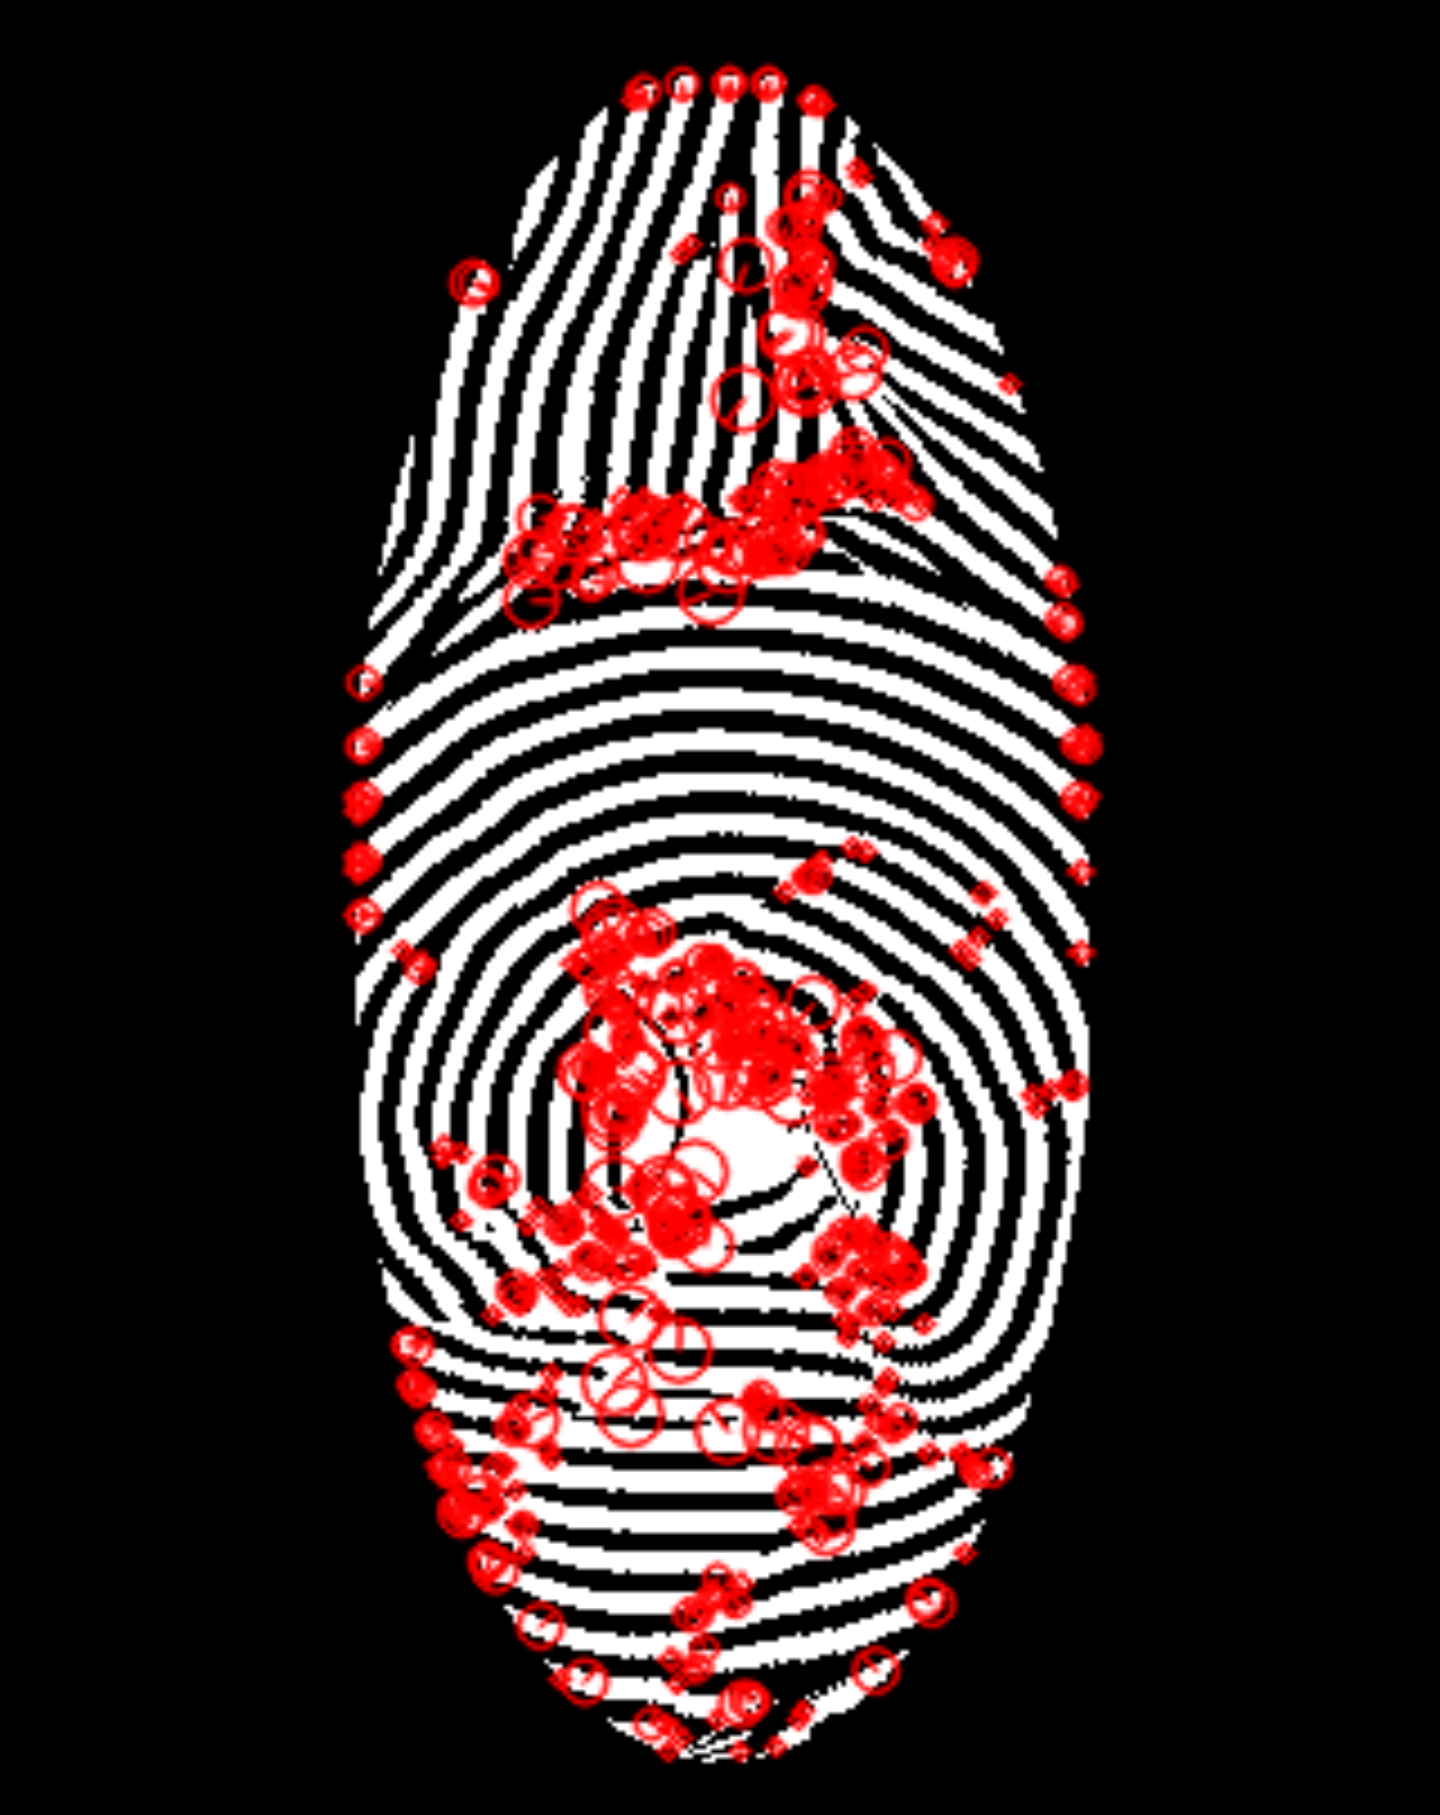
\includegraphics[width=.5\columnwidth]{assets/fingerprint}
	\caption{Extracted minutiae details from a fingerprint.}
	\label{fig:fingerprint}
\end{figure}

The procedure for fingerprint acquisition is divided in three steps.
First, a user opens the application on their smartphone and takes a photo of his or her finger inside an elliptic-shaped area.
Next, the captured photo is processed and analysed using various algorithms to extract minutiae fingerprint details.
This yields the data presented in Figure \ref{fig:fingerprint} where indicating feature points are indicated as small red dots.
Finally, the captured fingerprint is matched against known fingerprints available in the embedded database of the mobile device.
Smartphones such as the Google Pixel which are equipped with 128GB of storage space, can store up to ten million fingerprints.

After conducting a small experiment with our prototype, we conclude that the mean fingerprint matching accuracy is 55\% with the highest value of 67\% for thumb fingers.
These experimental results show that there is definitely room for improvement during the fingerprint processing and matching stages, however, we demonstrated the feasibility of this approach.
The ability to capture, process and match fingerprints in mere seconds, renders this concept usable in various scenarios like in remote regions with limited Internet connectivity.
This work provides a solution for portable trust and our framework has been specifically designed to serve as a building block for a self-sovereign identity solution.

\subsection{Self-sovereign Identity}

Most identity services are offered by a single authority, handing out, revoking and managing identities.
This trend continued when society adopted digital solutions: issuers of digital identities like Internet Assigned Numbers Authority (IANA) and Internet Corporation for Assigned Names and Numbers (ICANN), the organizations responsible for coordination of digital namespaces on the Internet, were and still are single, large organizations that have a large influence on the layout of the Internet landscape\footcite{pathtossi}.
Some identity schemes took a small step beyond a centralized structure and offered hierarchical solutions like certificate authorities (CAs).
However, such systems rely on root authorities which form a single point of failure.

As Internet usage increased, more and more digital services became available with the need for users to create their digital identity.
This resulted in identity fragmentation where a user had to manage multiple identities for different services, sometimes closely related.
User-centric Initiatives like OpenID, Facebook Connect and OAuth attempted to address this problem by providing a single identity service.
Digital service providers are able to implement such identity services without much effort to allow users to use only one shared identity.
Unfortunately, this type of identification is again regulated by mostly centralized authorities like Facebook or Google.
In addition, identity service providers are able to track users across different digital services.

While some of the described identity solutions are used by millions of users, they do not put the user owning that specific identity in control.
Another issue is that companies often want users to reveal more information about their identity than they actually need.
Sometimes, this data is used for analysis of user behaviour or data mining.
This raises the question whether an identity system can be designed, void of any central authority and where users can decide which attributes they wish to reveal.
Entities in need of identity information should be able to verify statements without being dependent on a central authority.

We present a Self-Sovereign Identity (SSI) mechanism, capable of verifying statements, without any central organization, point-of-failure or possibility of data tracking, giving users full control over their identity.
Self-sovereign identity serves a purpose in a large range of applications, have the potential to speed up traditional, inefficient verification processes and enables inter-operability between companies, individuals and governments while respecting the privacy of identity owners.
In a SSI system, civilians, legal entities and objects are able to prove statements such as "my age is at least 18" to others that legally require verification of this claim, like alcoholic shops or car rental services.
A reliable SSI mechanism is an indispensable building block to empower blockchain-based applications and sector-specific processes, operating at higher levels in our technology stack.

The only situation where the input of a centralized identity provider is required is when bootstrapping an identity.
Since a cryptographic key on itself does not have much legal basis, the identity should be endorsed by a public authority, like a government.
Our proposed SSI mechanism consists of two type of actors: attestors and challengers.
Attestors provide an attestation for a certain attribute, possibly for a (small) fee.
Challengers wish to prove the validity of a specific statement of the identity owner.
It is helpful to make attributes checked by challengers publicly available on a blockchain construction (discussed in Section \ref{sec:trustchain}); this allows others to find challengers that have knowledge about a specific attribute.

In our system, attribute values are encrypted and never leave the encrypted domain.
Instead, all actions like statement validation and attestations are operations on encrypted data using homomorphic encryption.
Statement validation is a prime example of a Zero-Knowledge Proof in which the identity owner proves truth about a statement to a challenger, without actually revealing the exact value of the attribute in the statement.
This implies that an alcohol shop is able to verify that a customer reached the eligible age but is not exposed to the actual age of the customer.
The described system is in particular useful when trading in the programmable economy since sellers are able to specify trade-specific identity requirements that buyers have to meet before a transaction takes place (i.e. restrictions on age, residence or reputation).

\subsection{Blockchain Layer (TrustChain)}
\label{sec:trustchain}
The TrustChain transaction fabric is designed around the notion of entities performing transactions with each other.
Each user in the TrustChain network maintains and grows their own chain of historical transactions. 
This is in contrast to traditional blockchain constructions like Bitcoin or Ethereum, where a single, global ledger is maintained, containing all transactions since the inception of the platform.
We now discuss the creation, storage and dissemination of transactions recorded on TrustChain.

\begin{figure}[h!]
	\centering
	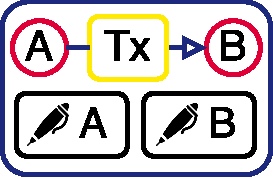
\includegraphics[width=0.3\columnwidth]{assets/trustchain_tutorial_1}
	\caption{A representation of a transaction between two users. When a transaction takes place, both involved parties digitally sign the transaction.}
	\label{fig:trustchain_tutorial_1}
\end{figure}

Imagine two users that are performing a transaction with each other.
This transaction can be transferral of money, exchanging data, attribute attestation or ownership transferral of a specific asset.
Figure \ref{fig:trustchain_tutorial_1} shows a representation of a transaction between aforementioned users.
Both users digitally sign this transaction, acknowledging that they agree with the content of this record.
After the signatures are placed, both users persist the record to their local storage.

\begin{figure}[h!]
	\centering
	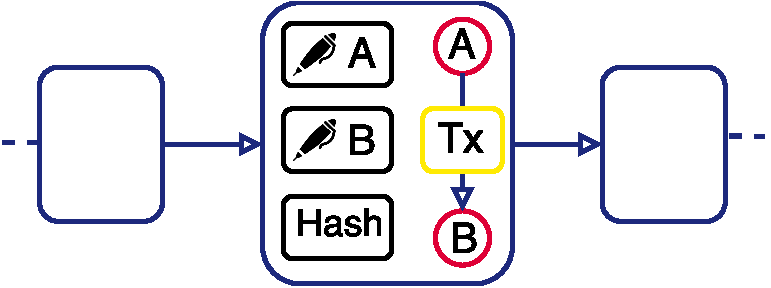
\includegraphics[width=0.7\columnwidth]{assets/trustchain_tutorial_2}
	\caption{A blockchain of transactions. Each block in the chain points back to the previous block.}
	\label{fig:trustchain_tutorial_2}
\end{figure}

A natural way to organize transactions is to chain them together.
Now, transactions are stored in a blockchain data structure where each block contains exactly one transaction, both signatures of the interacting participants and a pointer to the prior block in the chain.
To be precise, this pointer is a description of the previous block in the form of a digital hash (any secure hashing mechanism can be used for this purpose).
This idea is illustrated in Figure \ref{fig:trustchain_tutorial_2}.
Furthermore, each block is accompanied with a sequence number, uniquely identifying a specific block in the chain.
Each user creates a genesis block and keeps track of their own chain of transactions.
Every transaction block is present in the chain of both users involved in the transaction.

The data structure shown in Figure \ref{fig:trustchain_tutorial_2} is void of any control by other users. As a consequence, a user is able to tamper with their chain of transactions by inserting, removing or reordering records, without being noticed.
The integrity of this new transaction chain can be restored by recomputing all prior pointers.
In this situation, other users are unable to prove malicious modifications of one's chain.
Users might also decide to not append a transaction to their local chain which is tempting if the particular transaction has a negative impact on the standing of the user involved.

\begin{figure}[h!]
	\centering
	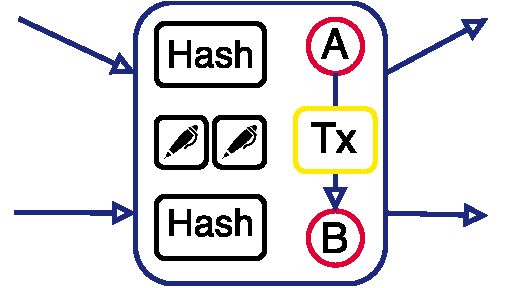
\includegraphics[width=0.5\columnwidth]{assets/trustchain_tutorial_3}
	\caption{To increase security, each block also references to a block in the chain of the other transaction participant. This ensures that each block has exactly two incoming and two outgoing pointers.}
	\label{fig:trustchain_tutorial_3}
\end{figure}

In TrustChain, this vulnerability is mitigated by adding an additional pointer in each block, see Figure \ref{fig:trustchain_tutorial_3}.
This pointer references to the prior block in the chain of the other transaction participant.
Now, when two users are interacting, their chains get intertwined or \enquote{entangled}.
This mechanism strengthens the tamper-proof property of TrustChain.
As presented in Figure \ref{fig:trustchain_tutorial_3}, each block has two incoming and two outgoing pointers.
Note that this scheme can easily be extended to support transactions between more than two participants, by increasing the amount of incoming and outgoing pointers of a block.

\begin{figure}[h!]
	\centering
	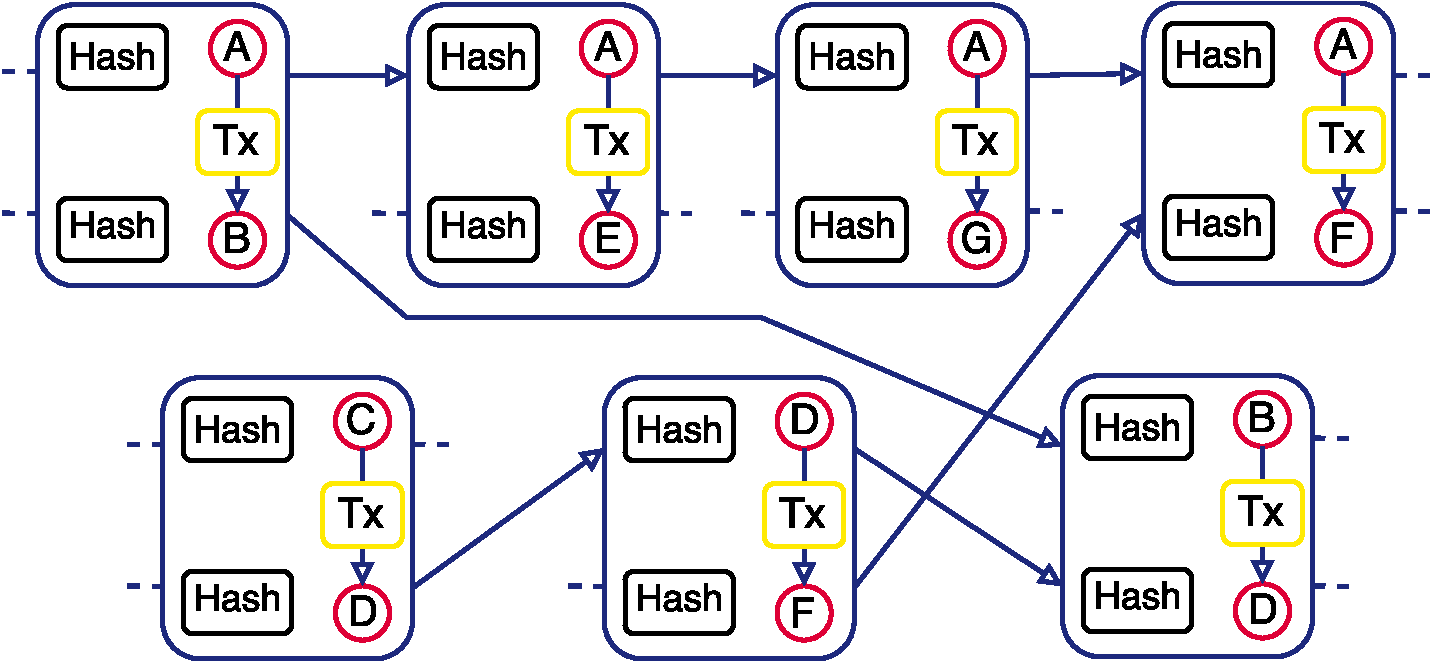
\includegraphics[width=0.9\columnwidth]{assets/trustchain}
	\caption{The tamper-proof TrustChain data structure to record transactions.}
	\label{fig:trustchain}
\end{figure}

As entities perform transactions with each other, they become quickly entangled with others.
Figure \ref{fig:trustchain} shows a part of the distributed TrustChain ledger where seven blocks, created by seven unique participants, are displayed.
Again, note that each block contains exactly two incoming and two outgoing pointers.

Before a new block is added to ones chain, a validation process takes place to verify the consistency and integrity of the local chain and the correctness of the new block.
This validation includes a verification of the pointers, transaction data, and signatures.
Only if the aforementioned checks pass, the block is appended to the chain, committed to the local storage and optionally shared with other users.

Our approach differs from traditional blockchain fabrics like Bitcoin or Ethereum in various ways.
Instead of a global, consistent and distributed ledger, every user maintains a personal history of interactions where in most blockchain-based systems, there exists one ledger which is acknowledged by a majority of the network participants.
Consistency of the global ledger is achieved by a consensus mechanism like proof-of-work or proof-of-stake.
While network consistency is essential for a cybercurrency system to prevent the double spending attack, it is not a hard requirement for a generic transaction ledger like TrustChain.
Some form of consensus is reached however, namely between the involved parties of a transaction.
We do not aim to prevent fraudulent operations but rather be able to detect malicious activities afterwards.
The absence of a global consensus mechanism allows for superior scalability with regard to transaction throughput since parallel transaction processing is inherently possible in TrustChain.
However, this does not mean that a consensus mechanism is not beneficial for TrustChain and as such, we present a novel consensus model in Section \ref{sec:scalable_consensus}.
Finally, at a minimum, network participants only have to store the transactions that they are involved in, significantly lowering the storage requirements compared to other blockchains.

TrustChain blocks are designed to be disseminated and replicated throughout the network.
In particular, this is important when transaction history is used as input for a reputation mechanism which needs the historical behaviour of others (see Section \ref{sec:reputation}).
Additionally, replication of blocks makes the system resistant against network churn where users go on- and offline at a fast rate.
Each user operates on their own bulk storage of blocks, resulting in partial storage of the global ledger.
Collecting information of other users is challenging due to the vulnerability to various attacks, their limited resources and the burst of their interactions.
Prior work investigates this problem and propose solutions for reliable and secure collection of the interaction history\footcite{gkoroureducing}.

We envision TrustChain as an essential building block in our programmable economy, providing the foundation for trustworthiness estimation and transaction recording.
The superior scalability and reduced storage requirements makes our transaction ledger suitable in the context of identity management and trading.

\subsection{Scalable Consensus}
\label{sec:scalable_consensus}
Most blockchain fabrics have a requirement for a consistent state which is agreed upon by (a part of) the network.
This requirement holds in particular when considering digital money (cybercurrencies) like Bitcoin or Ethereum.
Consensus of the global ledger is necessary to prevent the double-spending attack where users transfer the same digital asset twice in multiple transactions.
Possibility of such an attack impacts reliability and trust of the overall system, preventing community adoption.
Unfortunately, most consensus mechanisms are computationally expensive and limit the global transaction throughput of the system.
For instance, the proof-of-work consensus mechanism implemented in the Bitcoin fabric limits the theoretical transaction throughput to around seven transactions per second which is by far not enough for a medium to large-sized trading platform\footcite{duebitcoinscale}.
In comparison, Visa processes several hundreds of transactions every second and in April 2017, SWIFT recorded an average of 28.38 million payments per day or around 328 per second\footcite{visatransactions}\footcite{swifttransactions}.
This motivates the need for a scalable blockchain.

We designed, implemented and evaluated a fault-tolerant, horizontal scalable consensus mechanism on top of TrustChain, capable of detecting malicious activities performed by users like double-spending.
As far as the authors are aware, this is the first horizontal scalable blockchain fabric.
We built our system based on three important objectives:
\begin{itemize}
	\item Reaching global consensus on a global state: global consensus renders many types of malicious activities useless since the consistent state has consent of honest users in the network.
	\item Resistance against malicious users: our consensus mechanism should be unaffected by the presence of malicious users, with or without purpose attempting to manipulate the outcome of the global consensus. Usually, these attacks are successful when the amount of malicious users reach a specific threshold.
	\item Horizontal scalability: in this context, horizontal scalability means that as more users join the TrustChain network, the global transaction throughput increases. Note that the Bitcoin system is not horizontal scalable since the global transaction throughput is not dependent on the amount of users in the network.
\end{itemize}

\begin{figure}[t]
	\centering
	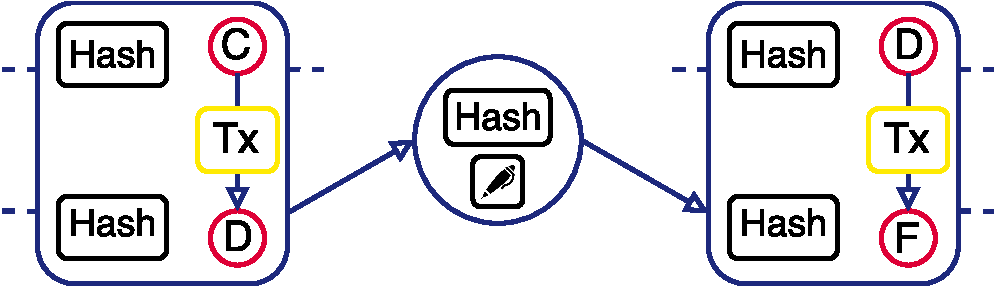
\includegraphics[width=0.8\columnwidth]{assets/trustchain_cp}
	\caption{The TrustChain structure extended with a checkpoint block. Each checkpoint block contains a signature of the user owning the chain and a hash of the consensus result.}
	\label{fig:trustchain_cp}
\end{figure}

First, the TrustChain data structure discussed in Section \ref{sec:trustchain} is slightly modified by adding a new type of block, called a checkpoint block.
This type of block is displayed in Figure \ref{fig:trustchain_cp}, presenting both a transaction block and a checkpoint block.
A checkpoint block consists of a pointer to a previous block in the same chain, a number indicating the round of the consensus mechanism after which the specific checkpoint block has been created, a cryptographic description of the result of the consensus and a digital signature, generated by the owner of the chain.
We modify the data structure such that the first block in a chain (the genesis block) is always a checkpoint block.
The checkpoint blocks in a chain are used during detection of malicious activities.

Our consensus mechanism proceeds in rounds and each round consists of two phases.
The outcome of each round is a set of checkpoint blocks agreed on by the facilitators of that round.
Facilitators are special user, elected during the first phase in a round of consensus.
These facilitators reach consensus not on the individual transactions like in Bitcoin or Ethereum but on the state of every chain.
If a specific user is not a facilitator, it sends its most recent checkpoint block to all facilitators.
When the facilitators received a sufficient number of checkpoint blocks, they start to reach consensus on all received checkpoint blocks using an Asynchronous Subset Consensus (ACS) algorithm\footcite{miller2016honey}.
When this algorithm is finished, the facilitators send two messages to all users, first the consensus result and second a signature message where the facilitator signed the consensus result, adding authenticity to the consensus result.
When a user receives the consensus result and a sufficient amount of valid facilitator signatures, a new checkpoint block is created and appended to the chain.
Finally, the new set of facilitators is elected and the round number is increased.
The process starts over now.

\subsection{TrustChain Experiments}
\label{sec:trustchain_experiments}
We have implemented TrustChain and the scalable consensus mechanism discussed in the previous sections.
This section will focus on experimentation to assess the global transaction throughput and consensus duration.
It is assumed that every user initiates two transactions per second.
We investigate the effect of varying the number of facilitators in the network; due to implementation-specific constraints, our network can host at most 32 facilitators.
The size of each transaction is approximately 500 bytes, resembling the average size of Bitcoin transactions.
This experiment is conducted on our DAS-5 supercomputer.

\begin{figure}[t]
	\centering
	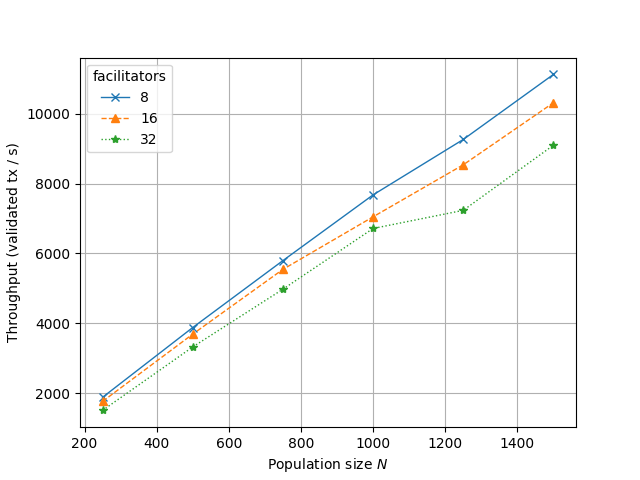
\includegraphics[width=0.7\columnwidth]{assets/trustchain_scalability}
	\caption{The TrustChain scalability experiment with a varying amount of facilitators. The horizontal axis indicates the number of users in the network and the vertical axis represents the global transaction throughput.}
	\label{fig:trustchain_scalability_experiment}
\end{figure}

The global throughput of TrustChain is displayed in Figure \ref{fig:trustchain_scalability_experiment}.
On the horizontal axis, the network size is shown as the amount of users whereas the vertical axis denotes the transaction throughput in transactions per second.
As a first observation, note the linear relationship in the figure between the amount of users in the network and the transaction throughput; this strongly indicates the horizontal scalability property for a network up to 1400 users.
The throughput rate lowers when the number of facilitators in increased. This is explained by the fact that more facilitators require additional network communication between users, introducing additional computational effort.

Figure \ref{fig:trustchain_scalability_experiment} indicates that we have indeed designed a scalable consensus mechanism, not bounded by a wasteful, expensive consensus mechanism like proof-of-work.
With only a few servers, our consensus mechanism is able to reach global throughput rates surpassing that of Visa or SWIFT.

\subsection{Trustworthiness and Reputation}
\label{sec:reputation}
One way to quantity trustworthiness in an economic system, is by using a reputation mechanism.
Reputation systems are widely used within the gig economy but the trust is often centred to a single authority.
Fifteen years of research on generic distributed reputation systems has yielded a wide variety of proposed designs and possible solutions\footcite{delaviz2010improving}\footcite{delaviz2012sybilres}\footcite{kamvar2003eigentrust}.
Prior work by us challenges the problem of estimating reputation using network flow algorithms.
This mechanism is called BarterCast and has been verified by a real-world implementation in our file-sharing software Tribler\footcite{meulpolder2009bartercast}.
The most challenging attack on decentralized reputation systems is the Sybil attack, where a malicious user manipulates his or her standing in the network by creating multiple fake identities (sybils) and initiating interactions with them.
To date, the Sybil attack remains largely unsolved and solutions that prevent manifestation such an attack, are often complex.

We have built and evaluated a distributed reputation mechanism, using irrefutable TrustChain records as foundation.
Building a reputation mechanism on top of TrustChain has several advantages.
First, TrustChain records are light-weight and designed to be exchanged with other users.
More importantly, the inherent tamper-proof property of TrustChain strengthens the reputation system since it becomes infeasible to tamper with past interactions.

Our reputation mechanism is based on PageRank, designed in 1998 by Larry Page and is called Temporal PageRank since it incorporates the notion of time\footcite{page1999pagerank}\footcite{otte2016sybil}.
PageRank is an accurate model that captures user behaviour when browsing the web and yields a ranking of websites based on relevance for that user.
The algorithm models websites and links between websites as a network and explores this network in a structured manner.
Temporal PageRank works in the same way, exploring the TrustChain data structure and analysing past transactions, including connections between them.
Additionally, it is a relatively simple and cheap technique from a computational perspective, requiring only minimal resources.
Temporal PageRank determines trustworthiness scores for other users from the perspective of a user performing the computation and is somewhat resistant against Sybil attacks in a sense that such attacks performed in the past only have minor influence on the outcome.

Temporal PageRank incorporates a weak form of transitive trust.
Transitive trust implies that trust is not only established between two entities but is transferred upon further interactions.
Specifically this indicates that if a specific entity A trusts another entity B well, he is also tempted to trust an entity C that is introduced to him by B.
This is a situation that occurs frequently in the real world since we are inclined to trust individuals introduced by a trustworthy entity.

\begin{figure}[t]
	\centering
	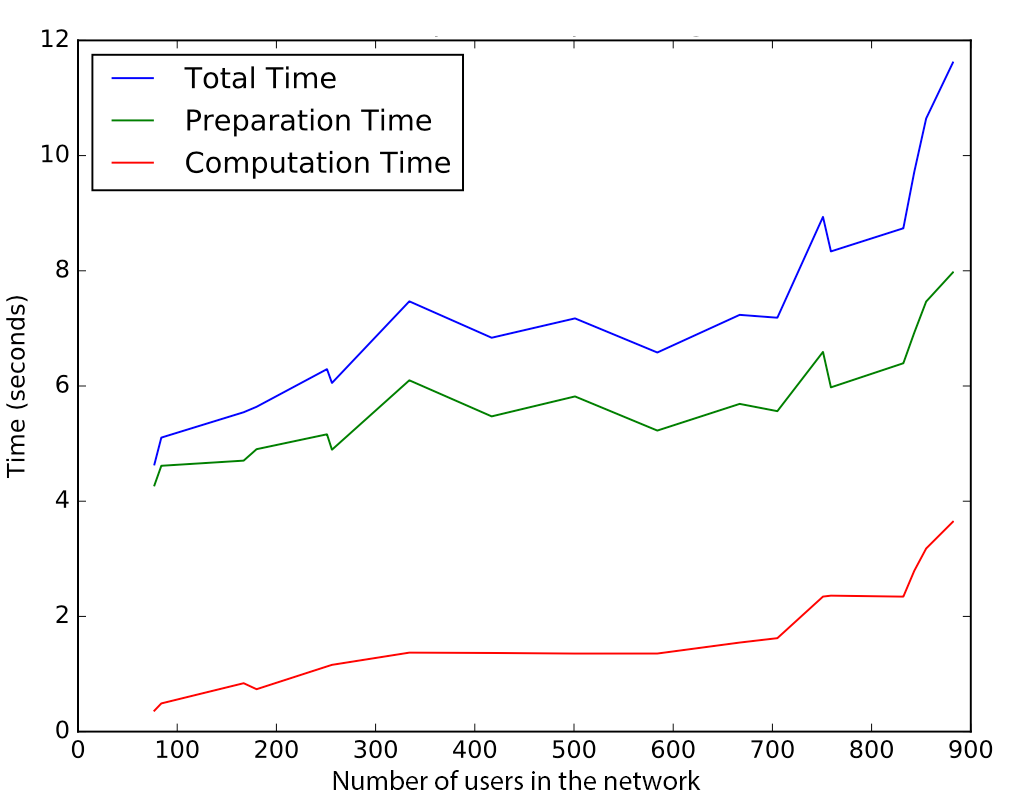
\includegraphics[width=0.6\columnwidth]{assets/pagerank_times}
	\caption{Performance of Temporal PageRank. The horizontal axis shows the number of users in the network and the vertical axis denotes the time it takes to estimate trustworthiness scores for all users in this network.}
	\label{fig:pagerank_performance}
\end{figure}

To demonstrate the feasibility of Temporal PageRank, we evaluated the mechanism using a real-world interaction trace, extracted from our file-sharing network Tribler for over a month.
This trace includes 917 unique identities and around 200.000 unique transactions.
The result of our experiment is displayed in Figure \ref{fig:pagerank_performance}.
The horizontal axis displays the number of users in the trace and the vertical axis shows the time it takes to compute a reputation score for all these users.
For a network with 900 identities, it seems that it takes just under 12 seconds to compute reputation scores.
It is often not necessary to determine reputation of all users in the network; in most scenarios, determining reputations of identities you are likely to interact with is sufficient.
However, we have demonstrated that Temporal PageRank is a feasible mechanism to use for trustworthiness estimation, even when the amount of users in the network grows.

\subsection{Real-time Clearance and Settlement}
\label{sec:internet_of_money}

\subsection{Decentralized Marketplace}

The final piece of our trust architecture is an operational prototype for a generic, decentralized two-sided marketplace, capable of trading generic assets like houses, currencies or bonds.
The platform facilitates trading without presence of a central clearinghouse performing matchmaking and processing trades.
Matchmaking, clearing and settlement proceeds in a completely decentralized fashion where autonomous entities are directly exchanging buy and sell offers.
Every trader operates on their own orderbook and acts as a matchmaker for others, attempting to match buy and sell offers.
Assets are stored in wallets which are used to query available balance or to transfer assets to others.
When a trade between market participants has been settled, the transaction details including the type, quantity and price of the exchanged assets are stored on TrustChain (see Section \ref{sec:trustchain}) and gossiped to other traders.
This transaction history is used as input for trust estimation (see Section \ref{sec:reputation}).
Our marketplace is secured against malicious behaviour and built to be operational in the presence of a large amount of traders.
Finally, our market is void of any transaction fee, enabling unrestricted and fair trading unlike most existing blockchain-based exchanges.

\begin{figure}[t]
	\centering
	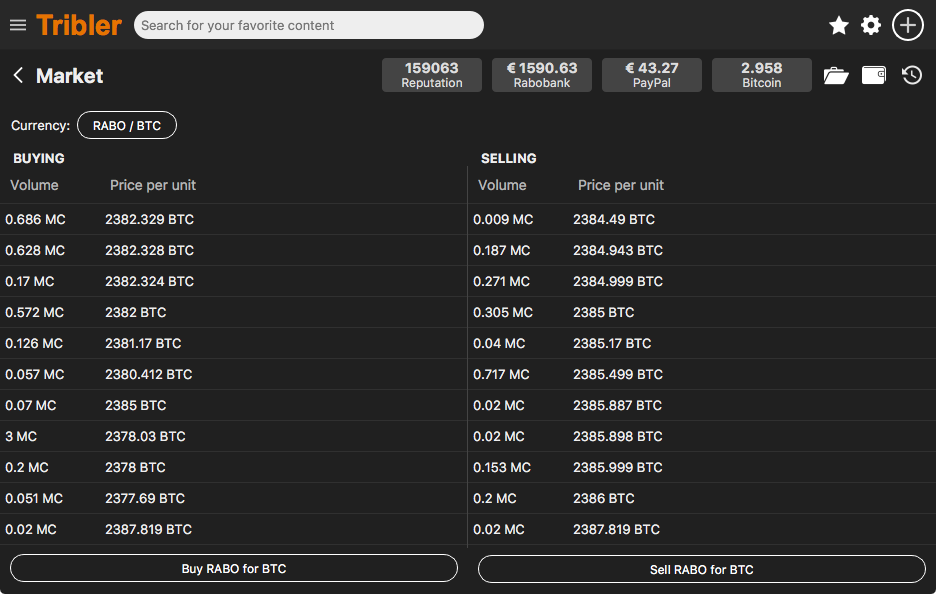
\includegraphics[width=.9\columnwidth]{assets/tribler_market}
	\caption{An orderbook on the decentralized marketplace, implemented in Tribler.}
	\label{fig:tribler_market}
\end{figure}

We built our decentralized marketplace and integrated it in Tribler.
The initial release of the marketplace supports trading bandwidth against both crypto- and regulated currencies, using the Internet-of-Money module discussed in Section \ref{sec:internet_of_money}.
Figure \ref{fig:tribler_market} shows the orderbook of a trader in the Tribler software.
Information about installed wallets of a trader are present in the upper-right corner of the window.

To obtain insight in the real-world efficiency of our system, we evaluate matching efficiency of Uber taxi drives.
Uber, one of the largest companies operating in the sharing economy, can be considered as a two-sided market where taxi drivers, offering a ride to a location, are matched against users requesting transportation.
Since there is no public, reliable dataset provided by the Uber platform, we use historical information of taxi rides published by the government of New York instead <ref>.
The dataset provides detailed temporal and geographical information of pick-up and drop-off location of each taxi ride.
We assume a total of 1100 taxi drivers and 1000 users requesting transportation.
It is also assumed that only the taxi drivers perform matching since they are likely to be connected to the network for a longer time whereas passengers most likely close the application when a taxi is available for them.
Taxi drivers and passengers are matched based on their geographical distance.

\begin{figure}[t]
	\centering
	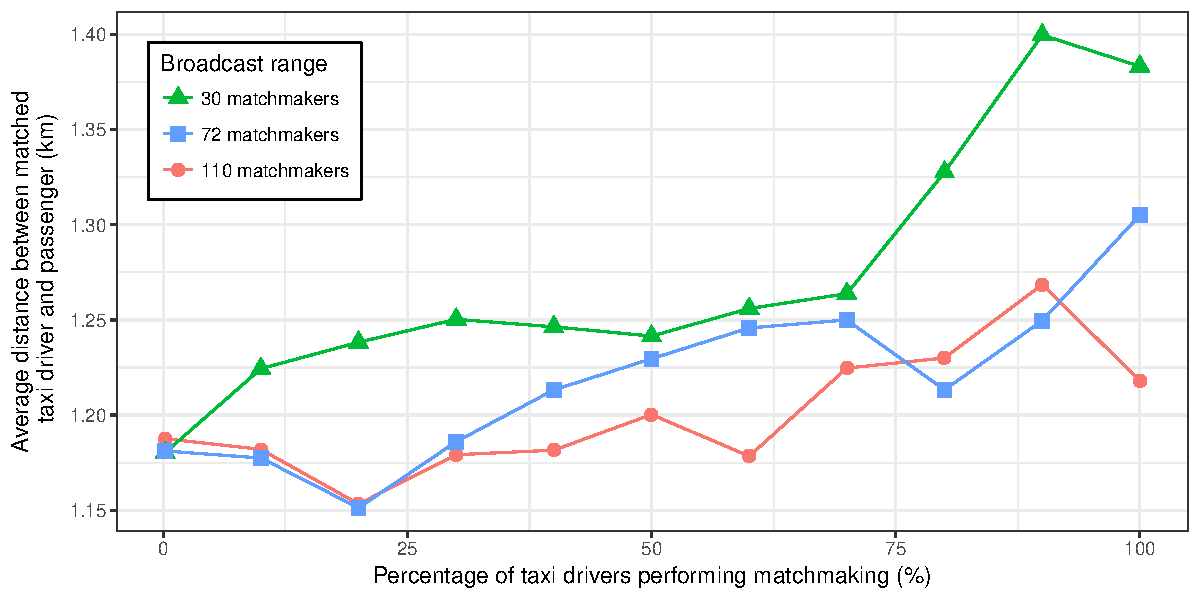
\includegraphics[width=0.8\columnwidth]{assets/matching_efficiency}
	\caption{The effect of decentralization on matching efficiency when emulating the taxi network of New York. The horizontal axis shows the percentage of taxi drivers performing matchmaking and the vertical axis denotes the average distance between matched taxi driver and passenger.}
	\label{fig:matching_efficiency}
\end{figure}

Figure \ref{fig:matching_efficiency} shows the relation between rate of decentralization and efficiency during our evaluation.
The horizontal axis denotes the percentage of taxi drivers performing matchmaking whereas the vertical axis represents the average distance between the matched driver and the requester.
The first data point in Figure \ref{fig:matching_efficiency} is equivalent to the situation where there is a central matching service, like Uber.
It is clear that decentralization negatively impacts matching efficiency which is expected since each matchmaker only holds partial knowledge of the global order book.
In particular, a matchmaker might not be aware of an offer that could improve his proposed matching.
This effect can be reduced by synchronizing orderbooks between matchmakers, at the cost of additional required network communication but increased matching efficiency.

\section{Conclusions}

Over the past few years, blockchain technology has attracted a significant amount of media attention.
The adoption and growth of blockchain-powered platforms like Ethereum and Bitcoin raised questions whether blockchain is able to provide value within economic processes like trading, banking and the value chain.
Besides illegal trading and various security weaknesses resulting in compromised digital assets, there are to date few real-world results demonstrating long-term viability of blockchain technology in our legal systems.
We believe this is caused by a fundamental lack of ties to any real-world, legal system.

We proposed a novel architecture to create trust.
Each component of our technology portfolio is designed and implemented based on the philosophy of the Internet itself: self-governance and loosly coupled autonomous systems, interacting with each other.
The essential technology to cultivate trust within our decentralized technology platform is TrustChain, a blockchain built around the notion of transacting real-world entities.
Viability of our proposed technology portfolio is demonstrated in the real-world, with running code.
Our aim is to adopt the programmable economy as a mean to decrease organizational barriers, increase trading efficiency and provide more transparancy and openness in existing and new economic ecosystems.


%\bibliographystyle{oscola}

\end{document}
